  \chapter{METODOLOGI}

% Ubah konten-konten berikut sesuai dengan isi dari metodologi

\section{Metode yang digunakan}

% Contoh input gambar dengan format *.jpg
\begin{figure} [ht] \centering
  % Nama dari file gambar yang diinputkan
  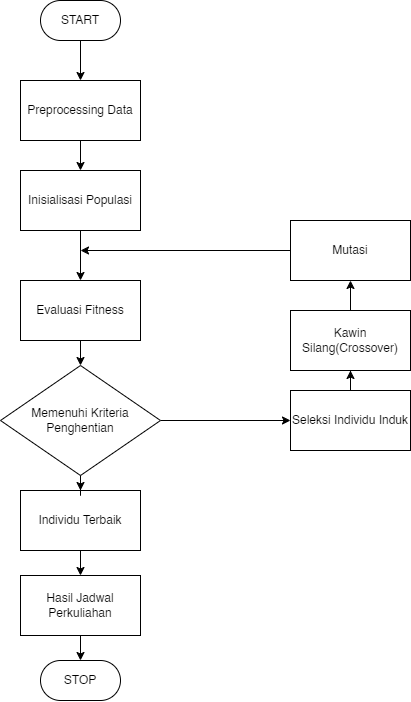
\includegraphics[scale=0.45]{gambar/Algoritma.png}
  % Keterangan gambar yang diinputkan
  \caption{Metodologi}
  % Label referensi dari gambar yang diinputkan
  \label{fig:Blueprint}
\end{figure}

% Contoh penggunaan referensi dari gambar yang diinputkan
Penulis akan menggunakan beberapa metode untuk menyelesaikan penelitian tersebut. 
Metode yang digunakan sebagai berikut:

\subsection{\emph{Preprocessing Data}}
  
  Pada penelitian ini, penulis akan menggunakan data dari Departemen Teknik Komputer ITS yang meliputi data mata kuliah, 
  jumlah ruangan, kapasitas masing-masing ruangan, jumlah dosen, dan jumlah mahasiswa. Data-data tersebut kemudian diolah 
  sedemikian rupa dengan metode encoding sehingga dihasilkan kromosom-kromosom yang akan digunakan sebagai induk dalam proses algoritma genetika.
  
\subsection{Inisialisasi Populasi}
  
  Individu-individu baru akan dibuat secara acak sesuai dengan desain kromosom yang telah dibuat sebelumnya.
  
  \subsection{Evaluasi Fitness}
  
  Individu dievaluasi dengan fungsi tertentu untuk menentukan kecocokan dengan batasan yang telah ditentukan sebelumnya. 
  Batasan-batasan tersebut dibagi menjadi 2 jenis yakni \emph{Hard Constraint} dan \emph{Soft Constraint.}
 
  \subsection{Pemilihan Indiidu Induk}
  
  Individu-individu yang telah melalui proses evaluasi dipilih untuk dijadikan sebagai induk untuk proses crossover. 
  Untuk memilihnya, dihitung probabilitas masing-masing individu dari nilai fitnessnya, kemudian dirandom menggunakan metode \emph{Roullete Wheel.}
 
  \subsection{\emph{Crossover}}
  
  Gen pada kromosom induk yang telah dipilih dipindah-silangkan sebagian antara satu dengan yang lain sehingga dihasilkan individu baru.

  \subsection{Mutasi}
  
  Setelah terbentuk individu baru, dilakukan perhitungan probabilitas mutasi untuk menentukan individu dan gen mana yang akan dimutasi. 
  Hasil dari mutasi ini akan dievaluasi nilai fitness nya untuk melihat apakah telah memenuhi kriteria atau belum. Kemudian proses akan berjalan lagi dari awal hingga memenuhi kriteria penghentian.
  
  \subsection{Kriteria Penghentian}
  
  Proses algoritma genetika hanya akan berhenti jika telah memenuhi kriteria penghentian yang telah ditentukan sebelumnya. 
  Kriteria penghentian ini dapat berupa nilai fitness tertentu, atau jumlah tertentu. 
  Jika nilai fitness telah terpenuhi atau jumlah iterasi telah terlewati, maka proses algoritma genetika akan berhenti.

\section{Bahan dan peralatan yang digunakan}
Dalam penelitian ini akan digunakan beberapa perangkat yang dibutuhkan untuk menunjang berjalannya penelitian dengan baik.
Berikut merupakan hardware dan software yang digunakan dalam melakukan proses pembuatan program sekaligus pengujian program yang digunakan pada penelitian ini.
\subsection{\emph{Hardware}}
Perangkat komputer yang digunakan untuk pengerjaan tugas akhir ini adalah \emph{Asus TUF FX 505 DT} dengan spesifikasi \emph{AMD Ryzen 5 R5-3550H Processor, GeForce GTX 1650 Graphics, 8GB DDR4, 1TB HDD,} dan \emph{Windows 10 64-bit}.
\subsection{\emph{Software}}
\emph{Software} yang digunakan dalam penelitian ini adalah Microsoft Visual Studio.


\section{Urutan pelaksanaan penelitian}

% Ubah tabel berikut sesuai dengan isi dari rencana kerja
\newcommand{\w}{}
\newcommand{\G}{\cellcolor{gray}}
\begin{table}[h!]
  \captionof{table}{Tabel timeline}
  \label{tbl:timeline}
  \begin{tabular}{|p{3.5cm}|c|c|c|c|c|c|c|c|c|c|c|c|c|c|c|c|}

    \hline
    \multirow{2}{*}{Kegiatan} & \multicolumn{16}{|c|}{Minggu} \\
    \cline{2-17} &
    1 & 2 & 3 & 4 & 5 & 6 & 7 & 8 & 9 & 10 & 11 & 12 & 13 & 14 & 15 & 16 \\
    \hline

    % Gunakan \G untuk mengisi sel dan \w untuk mengosongkan sel
    Studi Literatur &
    \G & \G & \w & \w & \w & \w & \w & \w & \w & \w & \w & \w & \w & \w & \w & \w \\
    \hline

    Pengumpulan Data &
    \w & \G & \G & \w & \w & \w & \w & \w & \w & \w & \w & \w & \w & \w & \w & \w \\
    \hline

    Preprocessing Data &
    \w & \w & \G & \G & \G & \w & \w & \w & \w & \w & \w & \w & \w & \w & \w & \w \\
    \hline

    Pembuatan Program &
    \w & \w & \w & \w & \G & \G & \G & \G & \G & \G & \G & \G & \w & \w & \w & \w \\
    \hline

    Pengujian Program &
    \w & \w & \w & \w & \w & \w & \w & \w & \w & \w & \w & \G & \G & \G & \w & \w \\
    \hline

    Penyusunan \linebreak Laporan &
    \G & \G & \G & \G & \G & \G & \G & \G & \G & \G & \G & \G & \G & \G & \G & \G \\
    \hline

  \end{tabular}
<<<<<<< HEAD
  \captionof{table}{Tabel timeline}
  \label{tbl:timeline}
\end{table}
=======
\end{table}

Pada \emph{timeline} yang tertera di Tabel \ref{tbl:timeline} \lipsum[10]
>>>>>>> f57e126874d0e1c43c733bfa968b0cb0f430594e
